%%%%%%%%%%%%%%%%%%%%%%%%%%%%%%%%%%%%%%%%%%%%%%%%%%%%%%%%%%%%%%%
% Plantilla Reporte Cientifico Paper Universidad del Azuay
% Creado por Darwin Darío Espinoza Saquicela
% Junio 2023
% IERSE -- Universidad del Azuay
%%%%%%%%%%%%%%%%%%%%%%%%%%%%%%%%%%%%%%%%%%%%%%%%%%%%%%%%%%%%%%%
\documentclass[a4paper]{article}
% Para ocultar los recuadros en referencias y links, agregar el parametro "hidelinks"

% Paquetes usados
%%%%%%%%%%%%%%%%%%%%%%%%%%%%%%%%%%%%%%%%%%%%%%%%%%%%%%%%%%%%%%%
\usepackage{fontspec}
\usepackage{hyperref}
\usepackage[titles]{tocloft}
\usepackage{apacite}
\usepackage{graphicx}
\usepackage{sectsty}
\usepackage{geometry}
\usepackage{ragged2e}
\usepackage{titlesec}
\usepackage{fancyhdr}
\usepackage{xcolor}
\usepackage{needspace}
\usepackage[absolute]{textpos}
\usepackage[spanish,mexico]{babel}
\usepackage{float}
\usepackage[section]{placeins}
\usepackage{tabularray}
\usepackage{booktabs}
\usepackage{multirow}
\usepackage{amsmath,empheq}
\usepackage{pdfpages}
\usepackage{lipsum}     % Generar texto de ejemplo

\selectlanguage{spanish}
\setmainfont{Times New Roman}
\title{Identificación de patrones de movilidad urbana y su relación con variables meteorológicas registradas en el cantón Cuenca}
\author{Darwin Darío Espinoza Saquicela}
\date{\today}

%%%%%%%%%%%%%%%%%%%%%%%%%%%%%%%%%%%%%%%%%%%%%%%%%%%%%%%%%%%%%%%
% Margenes -- Configuracion de pagina
%%%%%%%%%%%%%%%%%%%%%%%%%%%%%%%%%%%%%%%%%%%%%%%%%%%%%%%%%%%%%%%
\geometry{
  left=1.18in,   % Adjust the left margin
  right=1.18in,  % Adjust the right margin
  top=0.98in,    % Adjust the top margin
  bottom=0.98in,  % Adjust the bottom margin
}

%%%%%%%%%%%%%%%%%%%%%%%%%%%%%%%%%%%%%%%%%%%%%%%%%%%%%%%%%%%%%%%
% Especificar tamaños de fuente para comandos LateX
%%%%%%%%%%%%%%%%%%%%%%%%%%%%%%%%%%%%%%%%%%%%%%%%%%%%%%%%%%%%%%%
\makeatletter
\renewcommand{\huge}{\@setfontsize\huge{22}{26}}
\renewcommand{\Large}{\@setfontsize\Large{16}{19}}
\renewcommand{\large}{\@setfontsize\large{14pt}{17}}
\renewcommand{\small}{\@setfontsize\small{11pt}{13pt}}
\renewcommand{\normalsize}{%
    \@setfontsize\normalsize{12pt}{14.5}%
    \abovedisplayskip 10\p@ \@plus2\p@ \@minus5\p@
    \abovedisplayshortskip \z@ \@plus3\p@
    \belowdisplayshortskip 6\p@ \@plus3\p@ \@minus3\p@
    \belowdisplayskip \abovedisplayskip
    \let\@listi\@listI}
\makeatother

%%%%%%%%%%%%%%%%%%%%%%%%%%%%%%%%%%%%%%%%%%%%%%%%%%%%%%%%%%%%%%%
% Quitar numeracion de secciones, subsecciones y subsubsecc
%%%%%%%%%%%%%%%%%%%%%%%%%%%%%%%%%%%%%%%%%%%%%%%%%%%%%%%%%%%%%%%
\titleformat{\section}{\normalfont\Large\bfseries}{}{0pt}{}
\titleformat{\subsection}{\normalfont\large\bfseries}{}{0pt}{}
\titleformat{\subsubsection}{\normalfont\normalsize\bfseries}{}{0pt}{}

%%%%%%%%%%%%%%%%%%%%%%%%%%%%%%%%%%%%%%%%%%%%%%%%%%%%%%%%%%%%%%%
% Quitar numeracion de secciones, subsecciones y subsubsecc
% En tabla de contenidos
%%%%%%%%%%%%%%%%%%%%%%%%%%%%%%%%%%%%%%%%%%%%%%%%%%%%%%%%%%%%%%%
\renewcommand\numberline[1]{}
% Linea punteada para secciones
\renewcommand{\cftsecleader}{\cftdotfill{\cftdotsep}}

%%%%%%%%%%%%%%%%%%%%%%%%%%%%%%%%%%%%%%%%%%%%%%%%%%%%%%%%%%%%%%%
% Cabecera y pie de pagina
%%%%%%%%%%%%%%%%%%%%%%%%%%%%%%%%%%%%%%%%%%%%%%%%%%%%%%%%%%%%%%%
\definecolor{azulUDA}{HTML}{4472c4} % Color para elementos de pie de pagina
\fancyhf{}                          % Borrar cabecera/pie existente

% Cabecera de pagina
\rhead{
    \begin{textblock}{0}(11.3, 0.3)
        
\includegraphics[height=0.7in]{img/logo_posgrados23.jpg}
    \end{textblock}
}
\renewcommand{\headrulewidth}{0pt}  % Quitar linea vertical de la cabecera

% Pie de pagina
\lfoot{\textcolor{azulUDA}{Maestría en Matemática Aplicada}}
\rfoot{\textcolor{azulUDA}{Pág. \MakeUppercase{\thepage}}}
\renewcommand{\footrulewidth}{0.1pt} % Ancho de la linea horizontal
\renewcommand{\footrule}{\color{azulUDA}\hrule width\headwidth height\footrulewidth}

%%%%%%%%%%%%%%%%%%%%%%%%%%%%%%%%%%%%%%%%%%%%%%%%%%%%%%%%%%%%%%%
% Inicio de documento
%%%%%%%%%%%%%%%%%%%%%%%%%%%%%%%%%%%%%%%%%%%%%%%%%%%%%%%%%%%%%%%
\begin{document}

    % CARATULA
    %%%%%%%%%%%%%%%%%%%%%%%%%%%%%%%%%%%%%%%%%%%%%%%%%%%%%%%%%%%%%%%
    \newpage
\begin{titlepage}
    \begin{center}
         % LOGO UDA
        \begin{figure}[htb!]
        	\centering
        		
\includegraphics[height=1.17in]{img/logo_uda23.jpg}
        	\label{fig:logoUda2023}
        \end{figure}
        \vspace{1cm}
        
        % DEPARTAMENTO DE POSGRADOS
        \Large{\textbf{DEPARTAMENTO DE POSGRADOS}}\\
        \vspace{1.5cm}
        
        % TITULO DE PAPER
        \Large{\textbf{Título del trabajo de investigación escrito con una plantilla hecha en \LaTeX }}\\
        \vspace{2cm}
        
        % TITULO A RECIBIR
        \large{Trabajo de graduación previo a la obtención del título de:}\\
        \vspace{0.5cm}
        \large{\textbf{Magister en \LaTeX }}
        \vspace{1.5cm}

        % AUTOR
        \large{\textbf{Autor:}}\\
        \vspace{0.5cm}
        \large{Autor}\\
        \vspace{1.5cm}

        % DIRECTOR
        \large{\textbf{Director:}}\\
        \vspace{0.5cm}
        \large{Director}
        \vspace{1.5cm}

        % LUGAR Y FECHA
        \large{\textbf{Cuenca – Ecuador}}\\
        \vspace{0.5cm}
        % Año establecido por LateX
        \large{\textbf{\the\year}}
        \vspace{1cm}
    \end{center}
\end{titlepage}
    
    % Agradecimientos
    %%%%%%%%%%%%%%%%%%%%%%%%%%%%%%%%%%%%%%%%%%%%%%%%%%%%%%%%%%%%%%%
    \pagenumbering{roman}
    \newpage
    \pagestyle{fancy}
\begin{center}
    \vspace*{\fill} % Add vertical space and center content
        \begin{center} % Center the text
                \section*{\Large{\textbf{AGRADECIMIENTOS}}}
                \begin{justify}
                    \lipsum[1][1-10]\\
                \end{justify}
            
                \begin{justify}
                    \lipsum[1][1-8]\\
                \end{justify}
            
                \begin{flushright}
                    Autor
                \end{flushright}
        \end{center}
    \vfill % Add vertical space and center content
\end{center}
    
    % DEDICATORIA
    %%%%%%%%%%%%%%%%%%%%%%%%%%%%%%%%%%%%%%%%%%%%%%%%%%%%%%%%%%%%%%%
    \newpage
    \pagestyle{fancy}
\begin{center}
    \vspace*{\fill}
        \begin{center}
                \section*{\Large{\textbf{DEDICATORIA}}}
                \begin{justify}
                    \lipsum[2][1-10]\\
                \end{justify}

                \begin{justify}
                    \lipsum[2][1-9]\\
                \end{justify}
            
                \begin{flushright}
                    Autor
                \end{flushright}
        \end{center}
    \vfill % Add vertical space and center content
\end{center}
    
    % INDICE
    %%%%%%%%%%%%%%%%%%%%%%%%%%%%%%%%%%%%%%%%%%%%%%%%%%%%%%%%%%%%%%%
    \newpage
    \renewcommand\contentsname{ÍNDICE}
    \tableofcontents
    
    % INDICE DE FIGURAS
    %%%%%%%%%%%%%%%%%%%%%%%%%%%%%%%%%%%%%%%%%%%%%%%%%%%%%%%%%%%%%%%
    \newpage
    \renewcommand{\listfigurename}{ÍNDICE DE FIGURAS}
    \listoffigures
    
    % INDICE DE TABLAS
    %%%%%%%%%%%%%%%%%%%%%%%%%%%%%%%%%%%%%%%%%%%%%%%%%%%%%%%%%%%%%%%
    \newpage
    \renewcommand{\listtablename}{ÍNDICE DE TABLAS}
    \listoftables
    

    % TITULO DOCUMENTO
    %%%%%%%%%%%%%%%%%%%%%%%%%%%%%%%%%%%%%%%%%%%%%%%%%%%%%%%%%%%%%%%
    \newpage
    \pagenumbering{arabic}
    \pagestyle{fancy}

% TITULO DE ARTICULO
% ______________________________________________________________
\noindent\hrulefill
    \begin{center}
        \Large \textbf{Título del trabajo de investigación escrito con una plantilla hecha en \LaTeX\\}
        \vspace{0.5cm}
      
        \small Autor --
        \href{mailto:autorejemplo@es.uazuay.edu.ec}{autorejemplo@es.uazuay.edu.ec} \\
        Director --
        \href{mailto:directorejemplo@uazuay.edu.ec}{directorejemplo@uazuay.edu.ec}
    \end{center}
\hrulefill
% ______________________________________________________________

    % RESUMEN ESCRITO EN LATEX
    %%%%%%%%%%%%%%%%%%%%%%%%%%%%%%%%%%%%%%%%%%%%%%%%%%%%%%%%%%%%%%%
    \section{RESUMEN ESCRITO EN \LaTeX}

    \begin{justify}
        \lipsum[1-2][1-20]\\
    \end{justify}
    
    \begin{justify}
        \textbf{Palabras clave:} \lipsum[1][1] 
    \end{justify}
    \needspace{3\baselineskip} % Que existan al menos 3 espacios para ingresar seccion
    
    % ABSTRACT ESCRITO EN LATEX
    %%%%%%%%%%%%%%%%%%%%%%%%%%%%%%%%%%%%%%%%%%%%%%%%%%%%%%%%%%%%%%%
    \pagestyle{fancy}
\section{ABSTRACT ESCRITO EN \LaTeX}

    \begin{justify}
        \lipsum[1-2][1-20]\\
    \end{justify}
    
    \begin{justify}
        \textbf{Keywords:} \lipsum[1][1].
    \end{justify}
    \needspace{3\baselineskip}

    % RESUMEN Y ABSTRACT FIRMADO POR IDIOMAS DESDE PDF
    %%%%%%%%%%%%%%%%%%%%%%%%%%%%%%%%%%%%%%%%%%%%%%%%%%%%%%%%%%%%%%%
    \newpage
    \section{RESUMEN FIRMADO POR DPTO. DE IDIOMAS}
    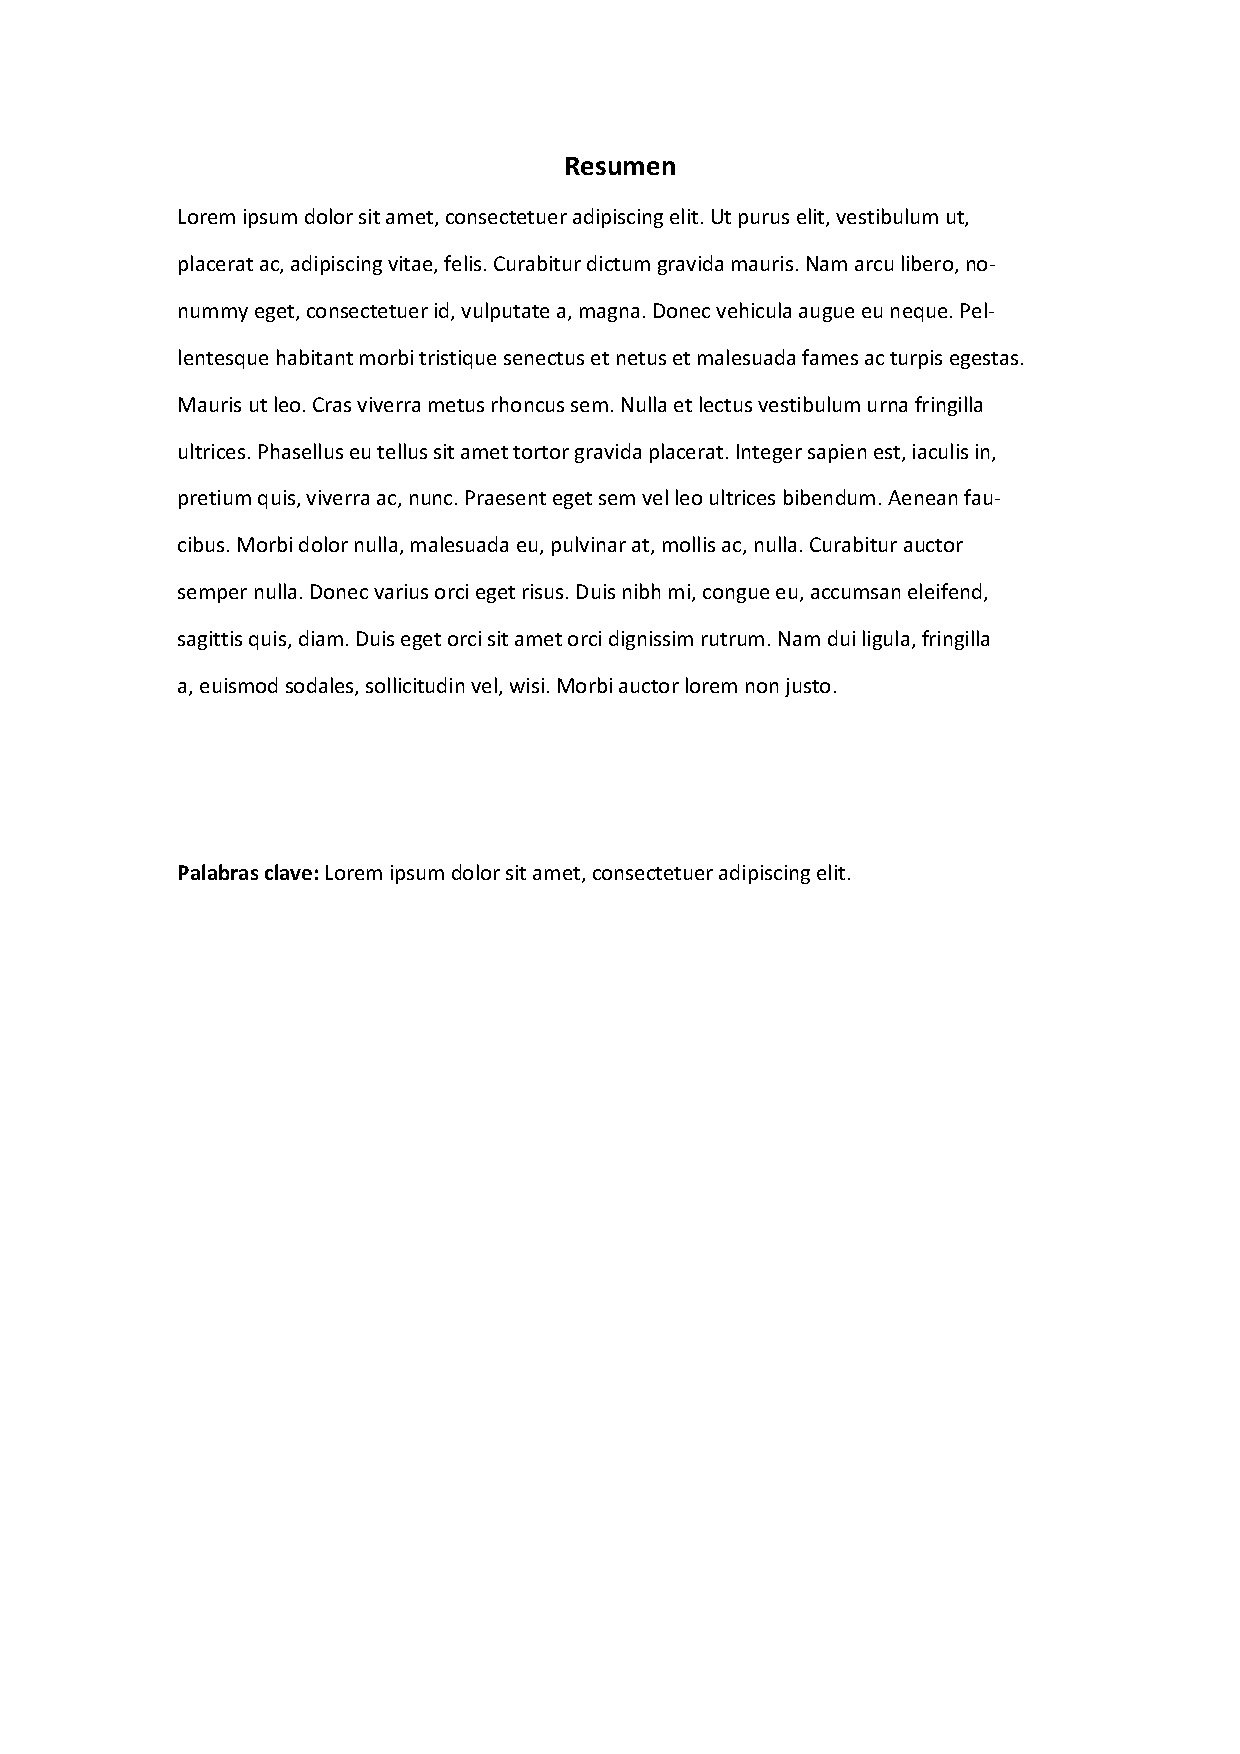
\includepdf[pages=1]{doc/resumen_asbstrac_idiomas.pdf}
    \newpage
    \section{ABSTRACT FIRMADO POR DPTO. DE IDIOMAS}
    \includepdf[pages=2]{doc/resumen_asbstrac_idiomas.pdf}
    
    % INTRODUCCION
    %%%%%%%%%%%%%%%%%%%%%%%%%%%%%%%%%%%%%%%%%%%%%%%%%%%%%%%%%%%%%%%
    \pagestyle{fancy}
\section{INTRODUCCIÓN}

    \begin{justify}
        \lipsum[1]\\
    \end{justify}
    
    \begin{justify}
        \lipsum[2]\\
    \end{justify}
    
    \begin{justify}
        \lipsum[3]\\
    \end{justify}
    \needspace{3\baselineskip}
    
    % REVISION BIBLIOGRAFICA
    %%%%%%%%%%%%%%%%%%%%%%%%%%%%%%%%%%%%%%%%%%%%%%%%%%%%%%%%%%%%%%%
    \pagestyle{fancy}
\subsection{Revisión bibliográfica}

    \begin{justify}
        \lipsum[1][1-10] \shortcite{example-article} \lipsum[2][1-15] \\
    \end{justify}
    
    \begin{justify}
        \lipsum[3][1-10] \shortcite{article1} \lipsum[4][1-15] \\
    \end{justify}
    
    \begin{justify}
        \lipsum[5][1-10] \shortcite{book1} \lipsum[6][1-15] \\
    \end{justify}
    \needspace{3\baselineskip}
    
    % METODOLOGIA
    %%%%%%%%%%%%%%%%%%%%%%%%%%%%%%%%%%%%%%%%%%%%%%%%%%%%%%%%%%%%%%%
    \pagestyle{fancy}
\section{METODOLOGÍA}

    \begin{justify}
        \lipsum[1] \\
    \end{justify}
    
    \begin{justify}
        \lipsum[2] \\
    \end{justify}

    \begin{justify}
        \lipsum[3][1-5] Figura \ref{fig:img_example} \lipsum[3][6-15] \\
    \end{justify}
    
    \begin{figure}[!ht]
        \centering
        
\includegraphics[scale=0.2]{img/default-image.jpg}
        \caption{\lipsum[1][1]}
        \label{fig:img_example}
    \end{figure}
    
    \subsection{Subsección 1}
    
    \subsubsection{Subsubsección 1}
    
    \begin{justify}
       \lipsum[4][1-5] Figura \ref{fig:img_example2} \lipsum[4][6-15] \\
    \end{justify}
    
    \begin{figure}[!ht]
        \centering
        
\includegraphics[scale=0.2]{img/default-image.jpg}
        \caption{\lipsum[2][1]}
        \label{fig:img_example2}
    \end{figure}
    
    \begin{justify}
        \lipsum[1][1-10] \shortcite{book1} \lipsum[1][1-15] \\
    \end{justify}

    \begin{enumerate}
        \item \lipsum[3][1]
        \item \lipsum[3][2]
        \item \lipsum[3][3]
        \item \lipsum[3][4]
    \end{enumerate}

    \begin{justify}
        \lipsum[1]\\
    \end{justify}
    \needspace{3\baselineskip}
    
    % RESULTADOS
    %%%%%%%%%%%%%%%%%%%%%%%%%%%%%%%%%%%%%%%%%%%%%%%%%%%%%%%%%%%%%%%
    \pagestyle{fancy}
\section{RESULTADOS}

    \subsection{
        Subseccion 2
        \label{analisys_ini}
    }
    
    \begin{justify}
        \lipsum[2][1-5] Figura \ref{fig:img_example3} \lipsum[2][6-15] \\
    \end{justify}
    
    \begin{figure}[!ht]
        \centering
        
\includegraphics[scale=0.2]{img/default-image.jpg}
        \caption{\lipsum[3][1]}
        \label{fig:img_example3}
    \end{figure}

    \begin{justify}
        \lipsum[1][1-5] Tabla \ref{tab:example_table} \lipsum[1][6-15] \\
    \end{justify}
    
    \begin{table}[htbp]
        \centering
            \begin{tabular}{|c|c|c|}
            \hline
            \textbf{Column 1} & \textbf{Column 2} & \textbf{Column 3} \\
            \hline
            Cell 1 & Cell 2 & Cell 3 \\
            \hline
            Cell 4 & Cell 5 & Cell 6 \\
            \hline
        \end{tabular}
        \caption{Tabla de Ejemplo Lipsum 1}
        \label{tab:example_table}
    \end{table}
    
    
    \begin{justify}
        \lipsum[6] Tabla \ref{tab:example_table2} \\
    \end{justify}

    \begin{table}[htbp]
        \centering
            \begin{tabular}{|c|c|c|}
            \hline
            \textbf{Column 1} & \textbf{Column 2} & \textbf{Column 3} \\
            \hline
            Cell 1 & Cell 2 & Cell 3 \\
            \hline
            Cell 4 & Cell 5 & Cell 6 \\
            \hline
        \end{tabular}
        \caption{Tabla de Ejemplo Lipsum 2}
        \label{tab:example_table2}
    \end{table}
    \needspace{3\baselineskip}
    
    % DISCUSION
    %%%%%%%%%%%%%%%%%%%%%%%%%%%%%%%%%%%%%%%%%%%%%%%%%%%%%%%%%%%%%%%
    \pagestyle{fancy}
\section{DISCUSIÓN}

    \begin{justify}
        \lipsum[1] \\
    \end{justify}
    
    \begin{justify}
        \lipsum[2][1-5] Tabla \ref{tab:example_table} \lipsum[2][6-10] \shortcite{example-article} \\
    \end{justify}
    
    \begin{justify}
        \lipsum[3] \\
    \end{justify}
    \needspace{3\baselineskip}
    
    % CONCLUSIONES
    %%%%%%%%%%%%%%%%%%%%%%%%%%%%%%%%%%%%%%%%%%%%%%%%%%%%%%%%%%%%%%%
    \pagestyle{fancy}
\section{CONCLUSIONES}

    \begin{justify}
        \lipsum[1] \\
    \end{justify}
    
    \begin{justify}
        \lipsum[3] \\
    \end{justify}
    \needspace{3\baselineskip}
    
    % REFERENCIAS
    %%%%%%%%%%%%%%%%%%%%%%%%%%%%%%%%%%%%%%%%%%%%%%%%%%%%%%%%%%%%%%%
    \renewcommand\refname{REFERENCIAS}
    \bibliographystyle{apacite} 
    \bibliography{mibibliografia}

\end{document}